\documentclass{article}

\usepackage{amsmath, amsthm, amssymb, amsfonts}
\usepackage{thmtools}
\usepackage{graphicx}
\usepackage{setspace}
\usepackage{geometry}
\usepackage{float}
\usepackage[hidelinks]{hyperref}
\usepackage[utf8]{inputenc}
\usepackage[spanish,es-nodecimaldot]{babel}
\usepackage{framed}
\usepackage[dvipsnames]{xcolor}
\usepackage{tcolorbox}
\usepackage{tikz}
\usepackage{caption}
\usepackage{longtable}
\usepackage{pdflscape}
\usepackage{svg}
\usepackage{subcaption}
\usepackage{caption}
\usepackage{multirow}
\usepackage{array}
\usepackage{listings}
\usepackage{cancel}
\usepackage{xurl}
\usepackage{import}
\usepackage{enumitem}

\colorlet{LightGray}{White!90!Periwinkle}
\colorlet{LightOrange}{Orange!15}
\colorlet{LightGreen}{Green!15}



\newcommand{\HRule}[1]{\rule{\linewidth}{#1}}

\declaretheoremstyle[name=Theorem,]{thmsty}
\declaretheorem[style=thmsty,numberwithin=section]{theorem}
\tcolorboxenvironment{theorem}{colback=LightGray}

\declaretheoremstyle[name=Proposition,]{prosty}
\declaretheorem[style=prosty,numberlike=theorem]{proposition}
\tcolorboxenvironment{proposition}{colback=LightOrange}

\declaretheoremstyle[name=Principle,]{prcpsty}
\declaretheorem[style=prcpsty,numberlike=theorem]{principle}
\tcolorboxenvironment{principle}{colback=LightGreen}

\newcolumntype{L}[1]{>{\raggedleft\let\newline\\\arraybackslash\hspace{0pt}}m{#1}}
\newcolumntype{C}[1]{>{\centering\let\newline\\\arraybackslash\hspace{0pt}}m{#1}}
\newcolumntype{R}[1]{>{\raggedright\let\newline\\\arraybackslash\hspace{0pt}}m{#1}}

\setstretch{1.2}
\geometry{
    textheight=9in,
    textwidth=5.5in,
    top=1in,
    headheight=12pt,
    headsep=25pt,
    footskip=30pt
}

\lstdefinestyle{bashstyle}{
    language=bash,
    basicstyle=\ttfamily,
    backgroundcolor=\color{gray!10},
    keywordstyle=\color{blue},
    commentstyle=\color{green!40!black},
    stringstyle=\color{red},
    showstringspaces=false,
    numbers=left,
    numberstyle=\tiny\color{gray},
    breaklines=true,
    breakatwhitespace=true,
    frame=tb,
    rulecolor=\color{black!70},
    framerule=0.5pt,
    tabsize=4,
    captionpos=b,
    morekeywords={nvm,pm2,serve,mkdir,source,bat,yt-dlp} % Add custom Bash keywords here
  }

\lstdefinestyle{pythonstyle}{
    language=Python,
    basicstyle=\ttfamily\small,              % Typewriter font, slightly smaller
    backgroundcolor=\color{gray!10},         % Light gray background
    keywordstyle=\color{blue}\bfseries,      % Keywords in bold blue
    commentstyle=\color{green!50!black}\itshape, % Comments in italic green
    stringstyle=\color{red!70!black},        % Strings in dark red
    showstringspaces=false,                  % No special marks for spaces
    numbers=left,                            % Line numbers on the left
    numberstyle=\tiny\color{gray},           % Line number style
    breaklines=true,                         % Break long lines
    breakatwhitespace=true,                  % Break at spaces when needed
    frame=tb,                                % Top and bottom border
    rulecolor=\color{black!40},              % Slightly lighter border
    framerule=0.5pt,                         % Thin frame
    tabsize=4,                               % Tab size
    captionpos=b,                            % Caption below the listing
    morekeywords={self,assert},              % Add extra keywords if needed
}

% ------------------------------------------------------------------------------

\begin{document}

% ------------------------------------------------------------------------------
% Cover Page and ToC
% ------------------------------------------------------------------------------

\title{ \normalsize \textsc{}
	\\ [2.0cm]
	\HRule{1.5pt} \\
	\LARGE \textbf{\uppercase{Documentación Técnica}
		\HRule{2.0pt} \\ [0.6cm] \LARGE{Universidad de Bogotá Jorge Tadeo Lozano} \vspace*{10\baselineskip}}
}
\date{}
\author{\textbf{Alvarado Becerra Ludwig} \\
  \textbf{Barrios Jiménes Johan Felipe} \\
  \textbf{Lis Cruz Nicolás} \\
  \textbf{Vera Soto Julián David}\\
  Arquitectura Empresarial - 20251S}

\maketitle
\thispagestyle{empty}
\newpage

\thispagestyle{empty}
\newpage
\setcounter{page}{1}

\tableofcontents

\newpage



\section{Transcripción de las entrevistas}

En la actividad de AVATA del curso \textit{Arquitectura Empresarial} (figura \ref{fig:avata}) se dejó un archivo comprimido \texttt{.rar} con la transcripción de las entrevistas junto con unas etiquetas de tiempo tal como se muestra en la figura \ref{fig:transcript}. El objetivo es el de tener estos textos de manera organizada para así poder diferenciar de los entrevistador(es) y el entrevistado. Para lograr esto se van a utilizar dos modelos de inteligencia artificial pre-entrenados; \textit{Pyannote.audio}\cite{Bredin23,Plaquet23}, encargado de segmentar el audio por \textit{speaker} capturando en qué instante de tiempo otra persona habla; \textit{Whisper}\cite{radford2022robustspeechrecognitionlargescale}, encargado de transcribir lo que dicen los \textit{speakers}.

\begin{figure}[ht]
  \centering
  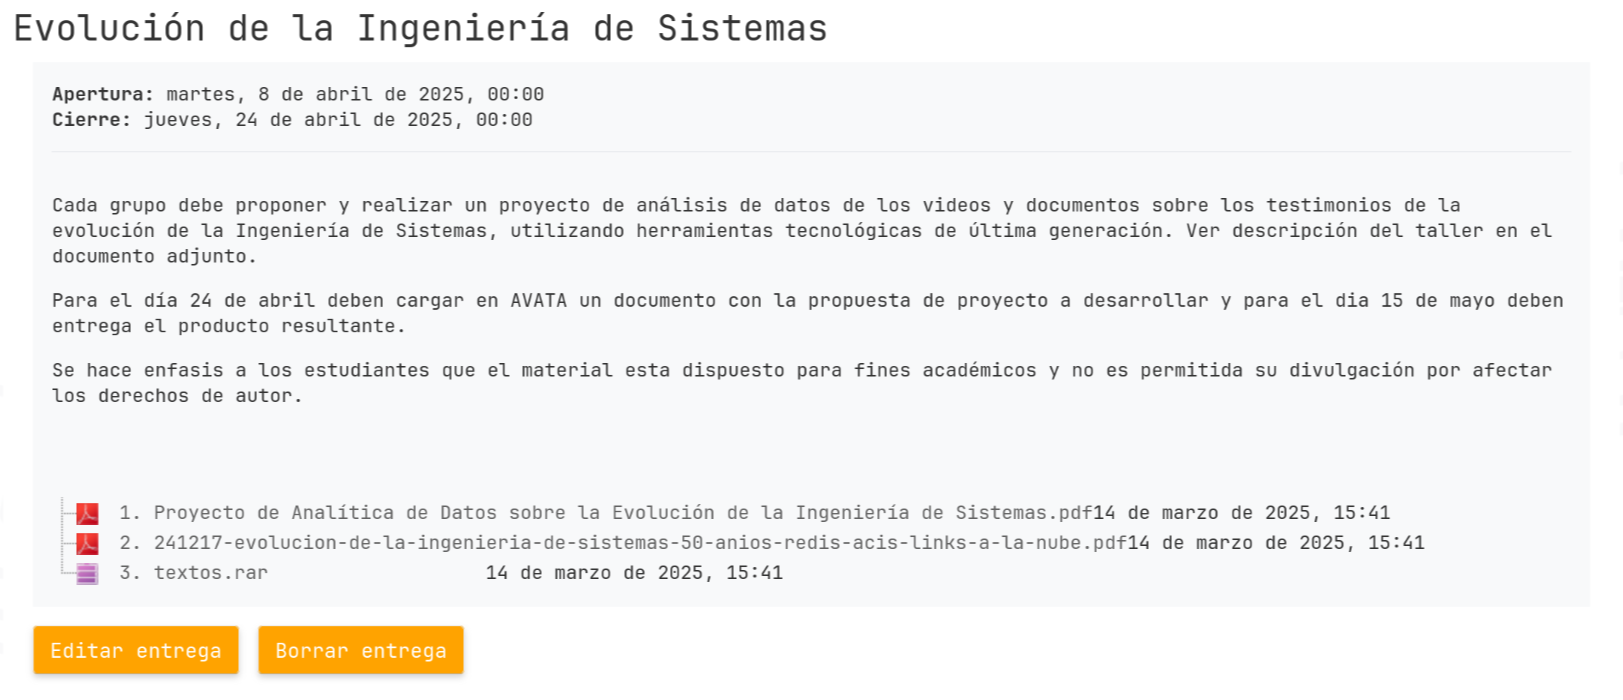
\includegraphics[width=\textwidth]{img/img1.png}
  \caption{\label{fig:avata} Actividad del curso junto con sus entregables y la transcripción de los textos.}
\end{figure}


\begin{figure}[ht]
  \centering
  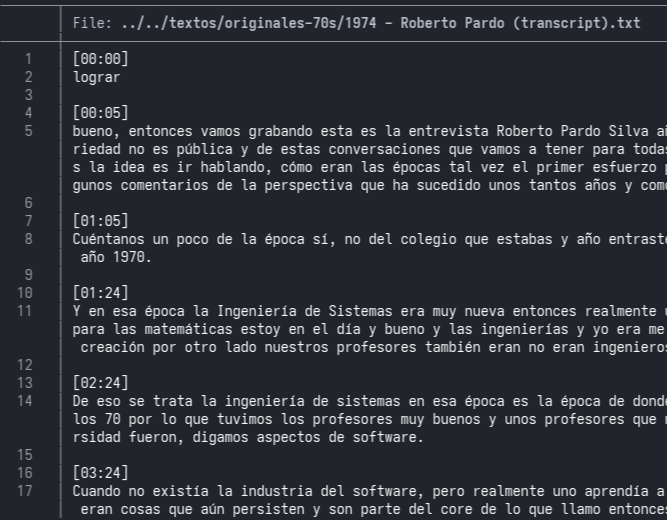
\includegraphics[width=0.5\textwidth]{img/img2.png}
  \caption{\label{fig:transcript} Ejecución del comando \lstinline[style=bashstyle]!bat 1974\ -\ Roberto\ Pardo\ \(transcript\).txt!  }
\end{figure}

\subsection{Descarga del audio}

Para poder obtener la transcripción completa de la entrevista se necesita de primero tener los audios de cada una de las entrevistas. Debido a que cada una de estas se encuentra en una lista de reproducción en la plataforma \textit{YouTube}\cite{youtube}. Los videos se pueden descargar con la herramienta \lstinline[style=bashstyle]!yt-dlp!, la cual, para el caso del encargado de esta tarea que está desde un computador GNU/Linux Arch, el paquete se puede instalar de la siguiente manera:

\begin{lstlisting}[style=bashstyle]
sudo pacman -S yt-dlp
\end{lstlisting}

Una vez obtenido el paquete se puede proceder a la descarga del audio de todos los videos que se encuentran en la lista de reproducción \url{https://www.youtube.com/playlist?list=PLH7DU-xDqcbejjNtxxIYDR9K5F1NYGi8L} ejecutando el siguiente comando:

\begin{lstlisting}[style=bashstyle]
yt-dlp -x --audio-format mp3 "https://www.youtube.com/playlist?list=PLH7DU-xDqcbejjNtxxIYDR9K5F1NYGi8L" 
\end{lstlisting}

Después de hacer la ejecución se descargan en audio \texttt{mp3} las 23 entrevistas, la salida deberá verse parecida a la figura

\begin{figure}[ht]
  \centering
  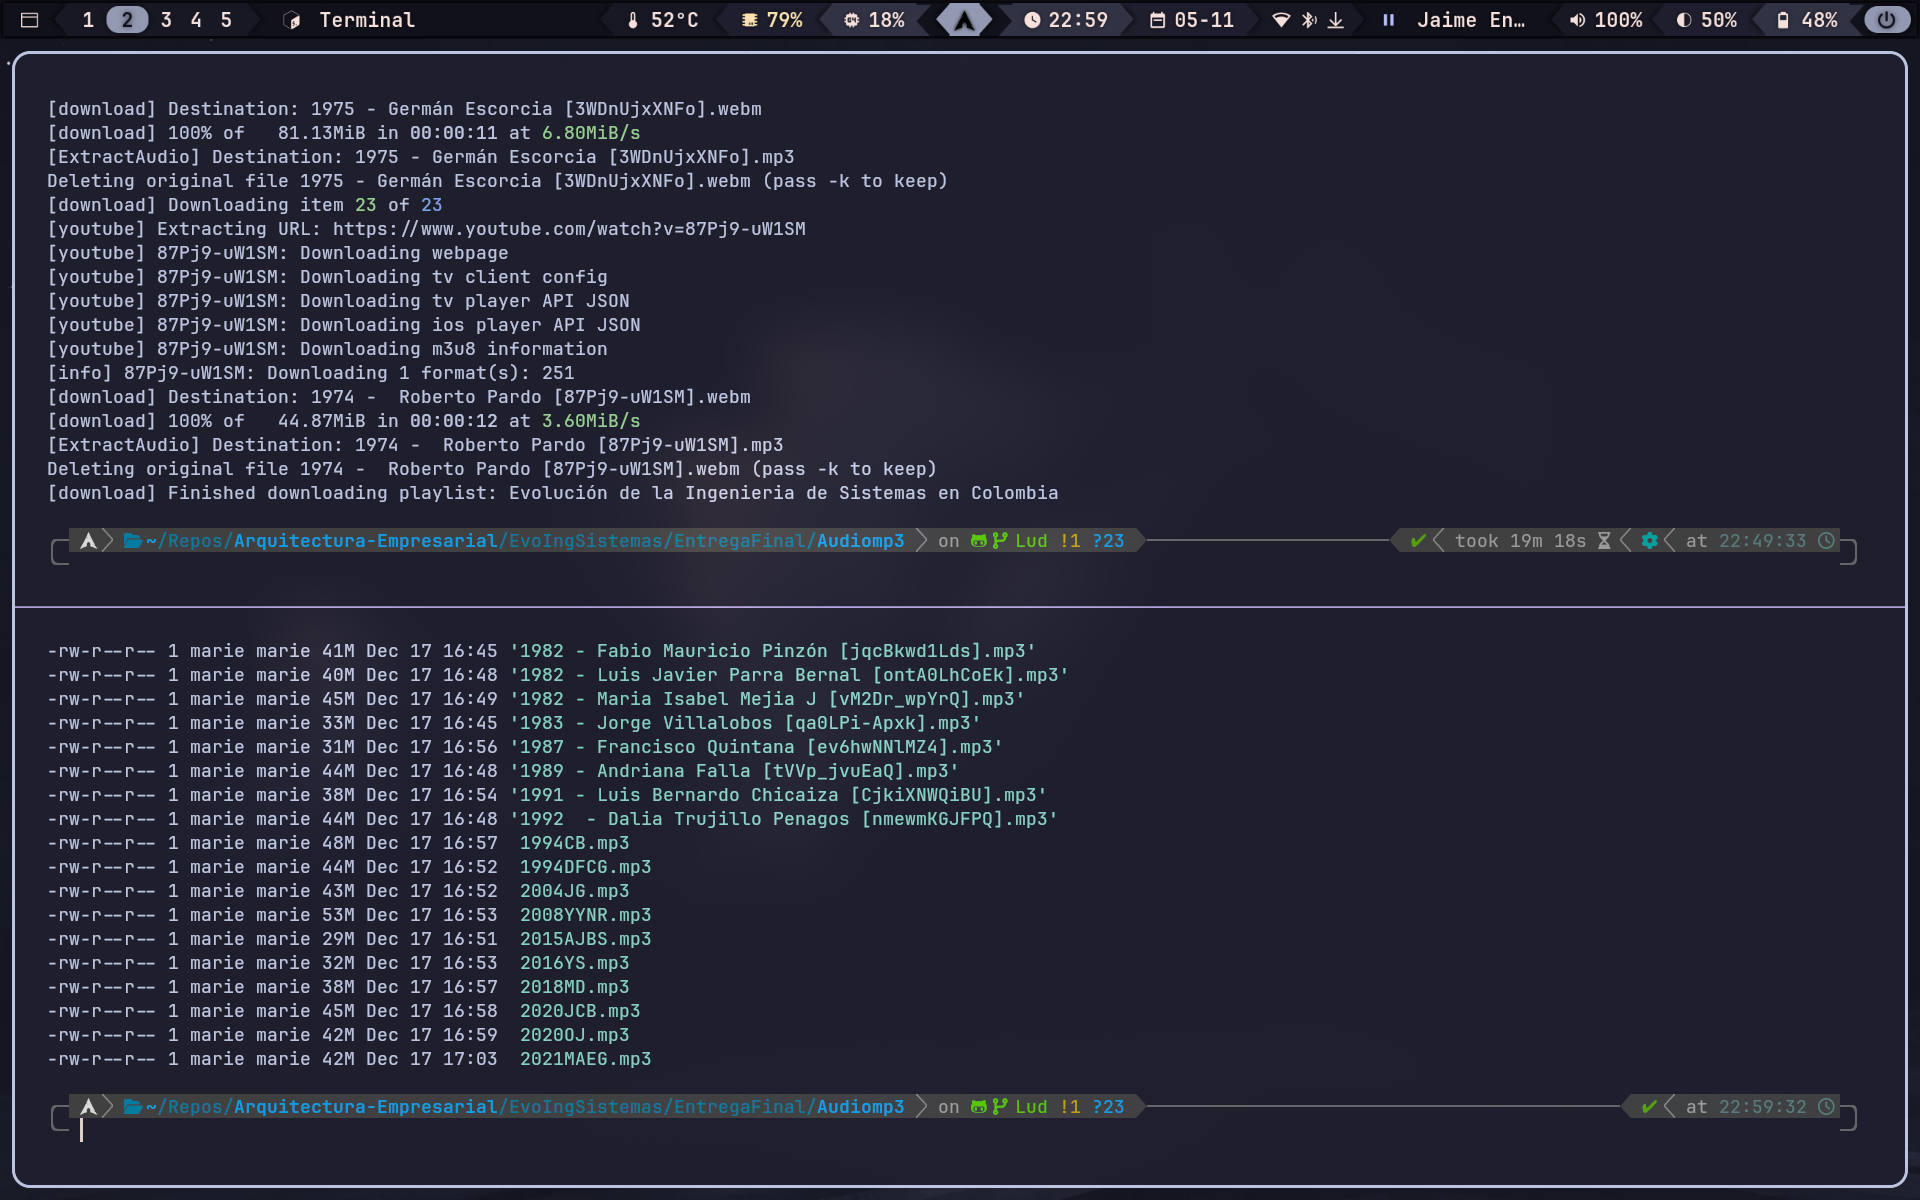
\includegraphics[width=0.5\textwidth]{img/OutputYT.png}
  \caption{\label{fig:yt-dlp} Descarga completada de todas las 23 entrevistas}
\end{figure}





\bibliographystyle{ieeetr}
\bibliography{referencias}


\end{document}
